\documentclass[11pt,letterpaper]{article}

\usepackage{amsfonts}
\usepackage{amsmath}
\usepackage{amssymb}
\usepackage[title]{appendix}
\usepackage{color}
\usepackage{csquotes}
\usepackage[margin=1in]{geometry}
\usepackage{graphicx}
\usepackage{listings}
\usepackage{multirow}
\usepackage{pifont}
\usepackage{tabularx}
    \newcolumntype{L}{>{\raggedright\arraybackslash}X}
\usepackage[usenames,dvipsnames,table]{xcolor}
\usepackage{xspace}
\usepackage{url}

\definecolor{cream}{RGB}{254,249,231}
\lstset{
    backgroundcolor=\color{cream},
    breaklines=true,
    basicstyle=\ttfamily\footnotesize,
    keepspaces=2,
    escapeinside={(*@}{@*)},
}

\newcommand{\parhead}[1]{\medskip \noindent \textbf{#1}~~}
\newenvironment{widelist}{\begin{list}{$\bullet$}{\setlength{\leftmargin}{.40cm}\setlength{\itemsep}{.00cm} }}{\end{list}}
\newcommand{\cmark}{\ding{108}}
\newcommand{\xmark}{ }
\newcommand{\pmark}{\ding{109}}
\newcommand{\name}{Phoenix\xspace}
\newcommand{\Name}{Phoenix\xspace}

\title{PhD Proposal}
\author{Stephen Herwig}
%\date{July 2, 2019}
\begin{document}
\maketitle
\begin{abstract}

Organizations shift the deployment of their services to untrusted third
parties, such as cloud infrastructures, content delivery networks, or email
providers, in order to reduce costs, increase availability, or gain
additional protections inherent to these hosting environments.
%
Unfortunately, such a shift poses a security tradeoff: third-parties that
provide or host the application potentially gain access to sensitive
information about the organization or its clients.


In my proposal, I ask whether it is possible to run legacy application binaries
with confidentiality and integrity guarantees that reflect the
organization's trust model with respect to the application and its
deployment setting.
%
The constraint of running unmodified, legacy applications implies that the
enforcement of such guarantees is the responsibilty of the applications's
run-time execution environment. 
%
Since the execution environment is transparent to the application, the insight
is that it may be modified, partitioned, and distributed across domains of
varying trustworthiness, so as to reflect the security goals.


In the first part of my proposal, I review my prior work in extending a
library operating system that runs within an Intel SGX secure hardware
enclave, so as to support running a broader set of trusted, legacy,
applications in untrusted environments.
%
In the second part, I propose a new run-time system, \emph{Gemini}, that is
agnostic to the availability of secure hardware and the trustworthiness of
the application.
%
Gemini presents two complementary abstractions: \emph{distributed containers},
where organizations pin sensitive data to domains that they trust, and
\emph{policy monitors}---modules that an organization installs in a trusted
environment to enforce expected behavior of untrusted applications.
%
I present the design of Gemini and propose a set of evaluations for assessing
its correctness and performance.

\end{abstract}

\section{Introduction}
\label{sec:intro}

Software is often written assuming monolithic trust assumptions, meaning that
the user tacitly trusts both the software and the environment in which it runs.
%
This assumption worked fine in the past, when an organization developed the
software, owned the infrastucture, and administered all parts of the resultant
system.
%
However, the trust assumption must be updated as new deployment scenarios bcome available.
%
A prime example is an organizations that outsources its services to untrusted
third parties, such as content delivery networks and mail providers.
%
Outsourcing is an attractive way for an organization to to reduce costs,
increase availabilty, or gain additional protections inherent to these hosting
environments.
%
Unfortunately, such a deployment poses a security tradeoff: the third party
providers that offer or deploy these services potentially gain access to
sensitive information about the organization and its clients, and the
organization may no longer have insight into what specific software is
implementing the service.


% TODO: maybe expand this paragraph a bit
%
% XXX: the problem is larger than just running trusted software on an untrusted
% host.
Running applications with strong security and privacy guarantees on untrusted
third parties is a large and active area of research; it spans uses of
trusted hardware and functional encryption that seek to continue hosting
applications completely on third parties, to (re-)designing applications and
protocols so as to delegate trust, preserve privacy, or otherwise partition
the application's execution across trust boundaries.
%
Unfortunately, this prior work either requires modifications to the
application, or has severe limits on the types of unmodified applications
supported.


% this is too specific
My thesis is:
\begin{displayquote}
    It is possible to run legacy application binaries with confidentiality and
    integrity guarantees that reflect the trust model in which the application
    is deployed.
\end{displayquote}
% Running unmodified, legacy binaries that have monolithic trust assumptions in
% environments where such assumptions do not hold.  

% For instance, an organization to outsource their unmodified, legacy, services
% to an untrusted hosting provider, who may in fact provide the service itself,
% without leaking private data to the provider and with guarantees that the
% provider does not deviate from the service's expected behavior.

The constraint of running unmodified, legacy services implies that the
enforcement of such security, privacy, and correctness guarantees is the
responsibilty of the service's run-time execution environment. 
%
Since the execution environment is transparent to the application, the insight
is that it may be modified, partitioned, and distributed across domains of
varying trustworthiness, so as to reflect the security goals of the
organization.


The design space is influenced by two factors: the presence of trusted
hardware, and the organization's trust in the application.
%
% Untrusted means the application may deviate arbitrarily from its stated
% purpose, subject to standard cryptographic assumptions, and, in particular, may
% actively try to leak sensitive data.
%
In my preliminary work, conclaves, I assume the presence of Intel SGX hardware
enclaves and that the content owners trust the service.
%
Conclaves extends prior work on SGX-based library operating systems (libOS) by
modifying a libOS to support running a broader set of legacy services
within enclaves: namely, multi-process, shared resource, applications.
%
% Specifically, conclaves is distributed system reminiscent of a microkernel,
% where each kernel service (for instance, a filesystem or shared memory)
% runs in a separate enclave and mediates the service’s shared resources
% among the application’s processes.


My proposed work, Gemini, makes assumptions about the availability of trusted
hardware and the trustworthiness of the application into policy specifications
on the part of the organization.
%
Gemini is an execution environment that offers two complementary abstractions:
(1) \emph{distributed container}, where organizations may pin sensitive data to hosts
that they trust; a thread's exeuction migrates to the trusted host when
computing with the sensitive data or any sensitive data derived from it, and
(2) \emph{policy monitors}, which are modules that an organization may installed in a
trusted environment that enforce expected behavior of untrusted application.
%
A key feature of policy monitors is that the policies enforce fine-grain
information flows.


To demonstrate this thesis, I make the following contributions:

This proposal is organized as follows:

% I evaluate my work by demonstrating correctness, measuring performance
% overheads, and measuring the “closeness” of the emergent protocols to proposed
% alternatives. I focus on the use cases of deploying TLS-enabled web services on
% content delivery networks (CDNs) without granting the CDN operator the private
% TLS key, as well as running database applications on untrusted third parties
% while maintaining the privacy of the database content.


% The conclaves
% paper is my "prior" work for this thesis, and the new work deals with migrating
% processes across trust domains (the unfinished work of a previous graduate
% student).




\section{Background}
\label{sec:background}

In this section, I clarify the problem with specific examples, and specifically
focuse on the everday case of outsourcing.
%
%
In this setting there are two principals: the \emph{organization} and the
\emph{cloud service provider}.
%
I describe the security and privacy implications of naively outsourcing, as
well as several trust models that apply to this setting, 
%
I then enumerate a list of goals for a system designed to handled these
implications.


\subsection{Problem}

There are two broad approaches of outsourcing.
%
The first, \emph{cloud hosting}, is an organization migrating its in-house
services to a third-party deployment; the second is an organization  migrating
from in-house services to those offered by third party \emph{cloud services}.
%
Hybrid approaches exist, such as where a cloud service provider must
communicate with the organization's, in-house, backend services.
%
Common outsourcing examples are an organization moving its HTTPS, DNS, or
email servers into the cloud, or contracting some other party to run its own
implementations of these services on the organization's behalf.
%
Nowadays, all of these core application-level protocols use public key
cryptography to ensure the integrity, authenticity, and/or confidentiality of
the application's content.


As a concrete example, consider an organization that outsources its web hosting
to a a content delivery network (CDN)\@.
%
A CDN is a massive, global network of \emph{edge servers}, where each edge
server acts as a reverse proxy for the organization: to
handle client requests, edge servers retrieve content from the organization's
\emph{origin servers}, and cache it so they can deliver it locally.
%
CDNs derive much of their utility from the fact that they have servers close to
most clients, thereby providing low-latency responses.
%
Several techniques exist for routing clients to the closest edge server, but
DNS is common, and so the CDN may also handle the organization's DNS server.
%
CDNs also provide added security benefits, such as absorbing DDoS
traffic, and filtering targeted malicious trafic, such as SQL injection and
cross-site scripting attacks~\cite{securing-cdns}.
%
Virtually all of the most popular websites (and a very long tail of unpopular
websites) use one or more CDNs to help reliably host their content.


With these use-cases in mind, let's enumerate the security and privacy
implications of outsourcing such service such services.


% XXX: try to keep each implication to one meaty paragraph.
\parhead{Impersonation}
% byzantine
%
In order for the provider to fulfill the service, the provider must
have access to the application's private keys.
%
Indeed, as the web moves towards HTTPS-everywhere~\cite{felt-2017-https},
organizations increasingly rely on CDN providers to store their HTTPS
certificate and the corresponding secret keys~\cite{key-sharing,
when-https-meets-cdn}, so that they can accept TLS connections while
maintaining low latency to clients.
%
Even with an application like DNS, where an organization would traditionally sign
its DNS records offline, the organization may choose to outsource the keys
and management to the provider.
%
% TODO: cite cloudflare blog
With the organization's private DNS keys online, the provider can offer
additional services, such as greater flexibility to return geographically-based
responses, as well as zone enumeration defenses.
%
This has significant implications on the trust model of each PKI and the web
writ large: today's providers can arbitrarily impersonate any of their customer
organizations.


\parhead{Breach of Confidentiality}
% Honest but curious
%
With the provider acting as a man-in-the-middle between the
organization and its clients, the provider is privy to the client's private
data, such as passwords, cookies, and personal content, as well as metadata 
for client profiling.
%
The provider might further subcontract aspects of the deployment (as with an
email provider using another provider for virus and spam scanning), with
the client and organization unaware of the extent of their data exposure.


\parhead{Correctness}
% concern 4: correctess: e.g., DNSSEC providers not actually providing DNSSEC.
% Negligent (also, a supertet of the byzantine and honest but curious)
%
By outsourcing a service, the organization no longer has guarantees that the
provider adheres to the expected service.
%
For instance, one DNS study~\cite{chung-2017-dnssec} discovered that 31\% of
domains that claim to support DNSSEC fail to publish all relevant records
required for a client resolver to validate the response, while
a study~\cite{open-http-proxies} of open HTTP proxies found that 5\% perform
unwanted or malicious content modification.


% TODO: call this something else
\parhead{Latent Trust Assumptions}
%
Assume a hybrid deployment where the organization has migrated its front-end
business applications to a cloud service provider, but that the application's
database remains within the organization’s network. 
%
Before migrating to the cloud, the database could trust that any connections to
it were from benign, internal tools; in the new deployment setting, the
organization must guard against potentially malicious or devious queries from
the cloud front-end.


\parhead{Legal and Regulatory Restrictions}
% concern 5: legal, policy compliance, ...restrictions
% talk about akamai not hosting content on thrid parties.
% talk about HIPPA (as with emails)
%
By outsourcing a service, the organization may be non-compliant with
industry regulations.
%
For instance, a hospital may be unable to run its electronic medical records
system in the cloud due to concerns  of HIPPA compliance.
%
In other words, even if the organization itself accepts the security and
privacy implications of outsourcing their services, legal matters may restrict
the degree to which the organization can leverage such deployments.


\subsection{Trust Model}

\begin{table}[t]
%\resizebox{.5\textwidth}{!}{
\small
\centering
\rowcolors{2}{gray!15}{white}
    \begin{tabular}{@{}lcccl@{}}
        & \textbf{Enclave}& \textbf{Provider} & \textbf{Software} & \textbf{Deployment} \\
        \hline
        1 & \cmark          &                   & \cmark          & Conclaves   \\
        2 &                 &                   & \cmark          & Gemini      \\
        3 & \cmark          &                   &                 & out of luck \\ % sandbox in enclave
        4 &                 &                   &                 & out of luck \\ % sandbox in partition
\end{tabular}
%}
\caption{The deployment strategy, depending on whether the provider offers
    trusted enclaves, whether the organization trusts the service provider, and
    whether the organization trusts the provider's application software.
    }
\label{tab:trust-models}
\end{table}

We describe an idealized trust model from the perspective of an
organization that uses a cloud service provider that requires the organization's
sensitive data.
%
For simplicity, we assume that the provider and the cloud machine owner are the
same party, and that the provider administers all software on the machine,
including any system software, such as the operating system, as well as the
application.
%
An untrusted provider may deviate arbitrarily from the stated service, but
remains subject to standard cryptographic assumptions.
%
Likewise, untrusted software may deviate abitrarily from its stated purpose
and, in particular, may actively try to leak sensitive data.
%
We assume, however, that the software is bug-free, and thus the model omits
external actors, such as a remote attacker.
%
The application may be composed entirely of open-source components, private
components that are proprietary to the provider, or some combination thereof.
%
If trusted boot is available  (either via a TPM, or in the form of secure
enclave launch), we assume that the organization and provider can agree to run
a specific build of system software, and that such software is trusted and
bug-free.


Table~\ref{tab:trust-models}, shows the different possible trust models based
on whether the provider offers hardware enclaves, whether the organization
trusts the provider, and whether the organization trusts the provider's
software.
%
We omit the uninteresting cases with a trusted provider, with the assumption
that the organization transitively trusts applications that the provider
offers.


In model 1, the organization trusts the software, but does not trust the
provider to run it faithfully, and thus uses one of various
approaches~\cite{talos,haven,scone,graphene} to
run an unmodified legacy application in an enclave.
%
This is the trust model for my prior work, conclaves, described in
\S\ref{sec:conclaves-summary}.
%
In contrast, in model 2, an enclave is not available (or assumed vulnerable to
to side-channnel attacks).
%
This is the starting use-case for Gemini, described in \S\ref{sec:gemini-design}.
%
In models 3 and 4, where neither the provider nor the software is trusted, no
general purpose solution exists for an organization to securely use an
commodity applicatins.


%For instance, the application may be composed of several components, some of
%which are trusted, and some are not; we assume that the organization
%trusts the components that interact with the senstive data.

In practice, the model's binary characterization of ``trusted" is too coarse,
the definition of untrusted as ``arbitrarily malicious" too strong,
and the assumptions of bug-free code and attacker-free environments too
naive.
%
For instance, it may be the case that most of the application is untrusted, but
the organization trusts a small portion of the application, such as its
cryptographic library.
%
This scenario is between models 2 and models 3 and 4, as the organization can
identify a small trusted computing base within the application.
%
Moreover, in the presence of attackers, an organization may simply
want strong, physical, isolation of its sensitive data from a remote attacker.
%
In other words, trust is a spectrum; the model highlights the endpoints of the
spectrums; my systems (conclaves and Gemini) target a specific endpoint, but,
to varying degress, allow for the relaxation of assumptions.



\subsection{Goals}

Our high-level goal is to allow the user to specify a trust policy to the
runtime execution environment; the runtime transparently implements the
policy on behalf of the applications.
%
I break down the policies into two categories:

\begin{widelist}
\item \textbf{Confidentiality policies:} Specifications of isolation boundaries for
    sensitive resources; the run-time constructs and enforces the boundaries.

\item \textbf{Integrity policies:} Specifications for data integrity; the run-time
    provides mechanisms for measuring integrity and detects breachs of
    integrity.
\end{widelist}


Our primary constraint is that the runtime should not require applications to be
rewritten or recompiled.
%
This is a practical constraint for system adoption, but also underscores our
thesis that such policies are deployment-specific, may be unknown during the
application's development, and must handle ``black box" applications, where the
source code is unavailable.
%
Our secondary constraint is that the policies should be simple; I want to avoid
degenerate solutions where the specification of the policy is more
onerous than simply rewriting the application.

Additional practical constraints, with respect to outsourcing, is that the policies
and runtime should handle applications that multiplex services across organizations,
with strong isolation between the organizations.
%
The system should also avoid degenerate solutions
that transfer undue hosting responsbilities back to the organization, thereby
defeating the intent of outsourcing.


Intuitively, the system will have worse performance than its vanilla
counterpart.
%
Nevertheless, the system should allow introspection into performance bottlenecks
as a means of investigating possible optimizations.


As non-goals, we are not concerned with obliviousness of the access paterns,
which may be a side-channel vector.

\section{Related Work}
\label{sec:related}

We present an overview of trusted execution environments, and then describe
three, not necessarily orthogonal techniques, for post-hoc adapting existing
software to satisfy alternative trust assumptions. 


\subsection{Trusted Execution Environments}

Trusted execution environments (TEEs) provide hardware protections for running
trusted portions of code with guarantees of confidentiality and integrity.  
%
Applications can be guaranteed that code executed within the TEE was run
correctly and that any secrets generated during execution will remain safely
within it as well.
%
A wide range of TEEs are available today, with varying functionalities.
%
We focus on Intel's Software Guard Extensions (SGX)\@.


\parhead{Intel SGX Overview}
%
Intel's SGX provides a new mechanism for trusted
hardware and software as an extension to the x86 instruction set~\cite{sgx,
mckeen2013innovative}.  
%
A program called an \textit{enclave} runs at high
privilege in isolation on the processor in order to provide trusted code
execution, while an untrusted application can make calls into the enclave.
%
While these enclaves can be statically disassembled (so the code running in the
enclave is not private), once an enclave is running, its internal state is
opaque to any observer (even one with physical access), as are any secrets generated.  


Enclaves must be measured and signed by their creator and cannot run without
this signature, and the enclave state is checked against this measurement
before running.  
%
An enclave can also cryptographically \textit{attest} to its current state, in
order to prove that it correctly executed code \cite{sgx_provisioning,
anati2013innovative}.  
%
Another feature is the ability to cryptographically \textit{seal} data to be
used across multiple invocations of an enclave~\cite{anati2013innovative,
sgx_sealing}.  
%
SGX also provides such features as trusted time and monotonic counters
\cite{sgx-linux-sdk,sgx-trusted-time}.  
%
However, as enclave code is always executed in user mode, system calls
must be proxied through the untrusted OS.


\parhead{AMD-SEV Overview}
%
%Whereas Intel SGX guards fine-grained units of execution, AMD's Secure
%Encryped Virtualization (SEV) is roughly the equivalent of an enclaved
%virtual machine.
%%
%SEV is based upon AMD Memory Encryption Technology, which introduces an
%AES-128 encryption engine inside the System on Chip (SoC) that transparently
%encrypts and decrypts the data when it leaves or enters the SoC, respectively.
%%
%Encryption key management, such as generating, storing, and delivering the
%keys, are carried out by the AMD secure processor and the encryption keys are kept
%hidden from untrusted parts of the platform.
%%
%The secure processor provides a set of APIs for provisioning and managing the
%platform in the cloud.
%
%
%SEV allows individual VMs to encrypt their memroy pages using their own secure
%keys; the VM's memory space is thus protected from from the hypervisor and
%co-resident VMs.
%%
%When code and data arrive into the SoC, SEV tags all of the code and data
%associated with the guest VM in the cache and limits access only to the tag's
%owner VM.
%%
%The guest OS is able to specify which memory pages are encrypted through new
%page table attributes.


\parhead{Attacks}
%
We must address the recent rise of side-channel attacks against SGX, including
the speculative execution attack Foreshadow~\cite{foreshadow,
weisse2018foreshadow}.  
%
This attack allows for the extraction of not only the entire SGX enclave's
memory contents but also the attestation and sealing keys.  
%
We note that this attack would break the security guarantees that we provide
with conclaves.
%
Intel has stated that SGX is explicitly designed to not deal with side-channel
attacks in its current state and leaves handling this up to enclave
developers~\cite{sgx-sidechannel, sgx-developers}.
%
Regardless, Intel has released both microcode patches and recommendations for
system level code that at the current time address Foreshadow and known related
attacks \cite{sgx-patch, canella2018systematic, weisse2018foreshadow}.  
%
There is also ongoing research to address both speculative execution as well as
other cache-based side-channel attacks on SGX and in general
\cite{yan2018invisispec, oleksenko2018varys, canella2018systematic, shih2017t}.

% TODO: add paragraph or two about attacks on SEV.


% Each solution operates at a differnet level in the stack, more or less.
% Handle TEE and non-TEE based solutions together.

\subsection{Partitioning applications across trust domains} 
% here, you can talk about program partitioning, both those that are aware of
% TEEs, and those that came before.


\parhead{Compiler Techniques}
%
Privtrans~\cite{privtrans} partitions a single program into two parts: a
privileged program called the monitor and an unprivileged program called the
slave. 
%
The monitor and slave run as separate processes, but communicate and cooperate
to perform the same function as the original program.
%
This is process-level isolation, and the monitor can be seen as interposing
between privileged operations and the main execution in the slave.


Privtrans allows a developer to add privilege separation to source code via
source-level annotations of variable and functions to indicate privileged
operations.  
%
Privtrans then propagates attributes, performs static analysis to find
privileged call sites, and performs C-to-C translation to partition the input
source code into the source code for the monitor and slave. 
%
Monitor must mediate access to all privileged resources, including the data
derived from such a resource; it is not sufficient for the monitor to only
perform access control.
%
In contrast, developers can augment monitors with application-specific
downgrade policies to make otherwise priviledged data flow from the monitor to
the slaves.  


\parhead{Protocol Refactoring}
%
Other work allows the organization to retain ownership of its private keys by
changing the server-side implementation of TLS\@.
%
SSL Splitting~\cite{ssl-splitting} leverages the fact that a TLS stream
comprises data records and authentication records (MACs), and develops a new
protocol in which the organization sends the authentication records and the
provider merges them with the data records to form the complete TLS stream.
%
Cloudflare's Keyless SSL~\cite{keyless-ssl} takes advantage of the fact that
TLS only uses the website's private key in a single step of the TLS handshake.
%
Like SSL Splitting, Keyless SSL keeps the master private key off of, and unknown
to, the proxy, but unlike SSL Splitting, Keyless SSL does not provide for
content provider endorsement of the content the proxy serves.  
%
Neither SSL splitting nor Keyless SSL provides for the protection of the
session keys from the provider.


\parhead{Virtualization Techniques} 
%
Several works~\cite{overshadow,inktag} that predate Intel SGX and AMD-SEV
extend the isolation capabilties of a hypervisor to give storng safety
guarantees to applications even in the presence of malicious guest operating
system.
%
These systems prevent the guest operating system from reading or modifying
application code, data, and registers through a technique called
\emph{cloaking}, in which the application sees a normal view of its memory
pages, but the OS an encrypted view.
%
Cloaking allows resources to remain accessible to the OS, yet secure,
permitting the OS to manage resources without compromising application
privacy or integrity.
%
Inktag also enables the hypervisor to verify the behavior of the untrusted
commodity operating system, as by checking that the memory mappings requested
by the application match those returned by the OS.


\subsection{Running (trusted) legacy applications in TEEs}
%
Various works use SGX as a mechanism for achieving shielded execution of
unmodified, trusted, legacy applications.
%
These works generally differ in how much of the application's code runs
within the enclave.


\parhead{Minimal TCB approachs}
%
At one extreme, TaLoS~\cite{talos} simply ports the LibreSSL library to SGX so
that the application terminates TLS connections in an enclave; the rest of
the application remains outside the enclave, unchanged.
%
% emphasize: smaller TCB, 
Several works~\cite{glamdring, panoply} generalize this approach by using developer
provided source-level annotations to partition an application into sensitive and
non-sensitive commponts, with the sensitive components running in an enclave.
%
In particular, Glamdring~\cite{glamdring} takes a similar approach to
Privtans~\cite{privtrans}, while also aiding a backslicing technique so that
fucntions and variables that influence a sensitive output are also isolated to
an enclave.  
%
Panoply~\cite{panoply} focuses less on the  partitioning scheme, but instead
allows the application to be partitioned into multiple enclaves, and
enforces run-time data and control flows between the resultant enclaves.


\parhead{Library Operating System Approaches}
%
At the other extreme, SCONE~\cite{scone} moves the entire C library into the enclave.
%
Haven~\cite{haven} and Graphene~\cite{graphene} carry this approach further by
implementing kernel functionality in an enclave by means of a library operating
system (libOS).  libOSes refactor a traditional OS kernel into a user-land
library that loads a program.
%
The program's C library is modified to redirect system calls to the libOS, which
in turn either services the calls internally or calls into the untrusted OS
when the host's resources are needed.
%
Aurora~\cite{liang2018aurora} extends the libOS from the SGX enclave to System
Management Mode (SMM) by running device drivers in SMM memory.


\subsection{Sandboxing (untrusted) applications via information flow controls}

\parhead{OS-Level IFC}
Decentralized information flow control (DIFC) enhanced operating systems allow
dynamic labeling of OS abstrations, such as processes and files, and enforce
access control based on Denning's lattic model for information flow
security~\cite{}.
%
The tags represent different rights (capabilities) with respect to the data
that the process is allowed to read or write.
%
Using tags, these systems can enforce the classical secrecy and integrity policies of
``no read up, no write down", or an integrity policy of ``no read down, no
write up", between the objects in the system.
%
Additional policies, such as \emph{export protection} are possible, in which a
process cannot have both an uncontrolled channel (e.g., a socket) open and
access to private data that it cannot declassify, as well as
policies for stringent system-wide \emph{read-protection} and \emph{integrity
protection}.
%
These process-level information flow models are coarse grained and cannot track
sensitive information \emph{within} untrusted applications.


\parhead{Fine-Grained IFC}
%
Fine-grained information flow tracking (IFT) is a technique whereby execution
runtime tags memory and registers containing sensitive data with labels (also
called taint or taint markings) and propagates these labels in
acccordance with the computation.
%
Instrumentation is transparent to the application process, as the application
observes the same addresses and same values as it would in an uninstrumented
execution.
%
IFT traditionally uses a source and sink model whereby labels are
assigned at sources and checked at sinks; the labels themselves are opaque,
and are interpreted by application-specific policy.
%
Most work in this area has been specifically motivated by detection of control
flow hijacking attacks, such as buffer overflows, and involves tainting of
program inputs, and trapping of control transfers to tainted target addresses.
%
However, IFT is also used to enforce mandatory access control on data and
derived data, and thus a restriction on the flow of information between
the system's objects (e.g., users, processes, files).


Fine-grained IFT can either be applied at the process- or system-level.
%
A standard approach for process-level information flow tracking is to run
the process in an emulator, such as Valgrind, Intel Pin, or DynamoRIO; the
emulator serves as a reference monitor, and dynamically tracks data flows.
%
In contrast, full-system IFT involves running the guest system in a hardware
emulator (e.g., QEMU) that has been augmented with machine instruction analysis
and taint tracking capabilities.
%
As an optimization, and for security isolation, a hypervisor may dynamically
switch execution between emulated execution when processing tainted data, and
native virtualized execution when processing untainted data.
%
Full-system IFT systems also propagate taint to the filesystem (as by storing
taint in a file's extended attributes) and across the network (as by placing
labels in a packet's IP options).


\parhead{Uses with Secure Hardware}
% TODO: also talk about compiler-based techniques (e.g., Moat)
%
Ryoan presents a request-response execution model that allows mutually
distrustful parties to process sensitive data in a distributed fashion on
untrusted infrastructure, without any party leaking secret data.
%
Ryoan runs each party's processing modules in a trusted userspace sandbox,
which in turn is hosted in an SGX enclave.
%
Each module tags its output, essentially performing taint tracking at
enclave-level granularity, where the taint indicates which encalves have seen
secret data.
%
When operating on tainted data, Ryoan ensures that the module cannot leak data
by controlling explicit I/O channels, obfuscating network traffic, forbidding
use of the fileystem, and ensuring that input is only processed once.


\section{Preliminary Work: Conclaves}
\label{sec:conclaves-summary}
%
% XXX: keep to ~4 pages

At a high level, our approach is to deploy applications in enclaves.
%
However, doing so in a manner that permits multi-tenancy and support
for legacy applications is challenging.
%
%
Recall from \S\ref{sec:sgxbackground} that libOSes expose traditional
OS kernel services within an enclave, and either handle the system calls
themselves or, when necessary (e.g., to send a network packet), hand
them off to the untrusted OS.
%
Conversely, we aim to be able to support dynamic scaling up and down of
web servers, tenant configurations, and security postures.

To address these challenges, we introduce a new architectural primitive that we
call a \emph{conclave}: in essence a container of enclaves.
%
As we will show, conclaves permit flexible deployment configurations and
achieve security in multi-tenant settings.


\subsection{Design and Implementation}

% Design diagram {{{

\begin{figure}
\centering
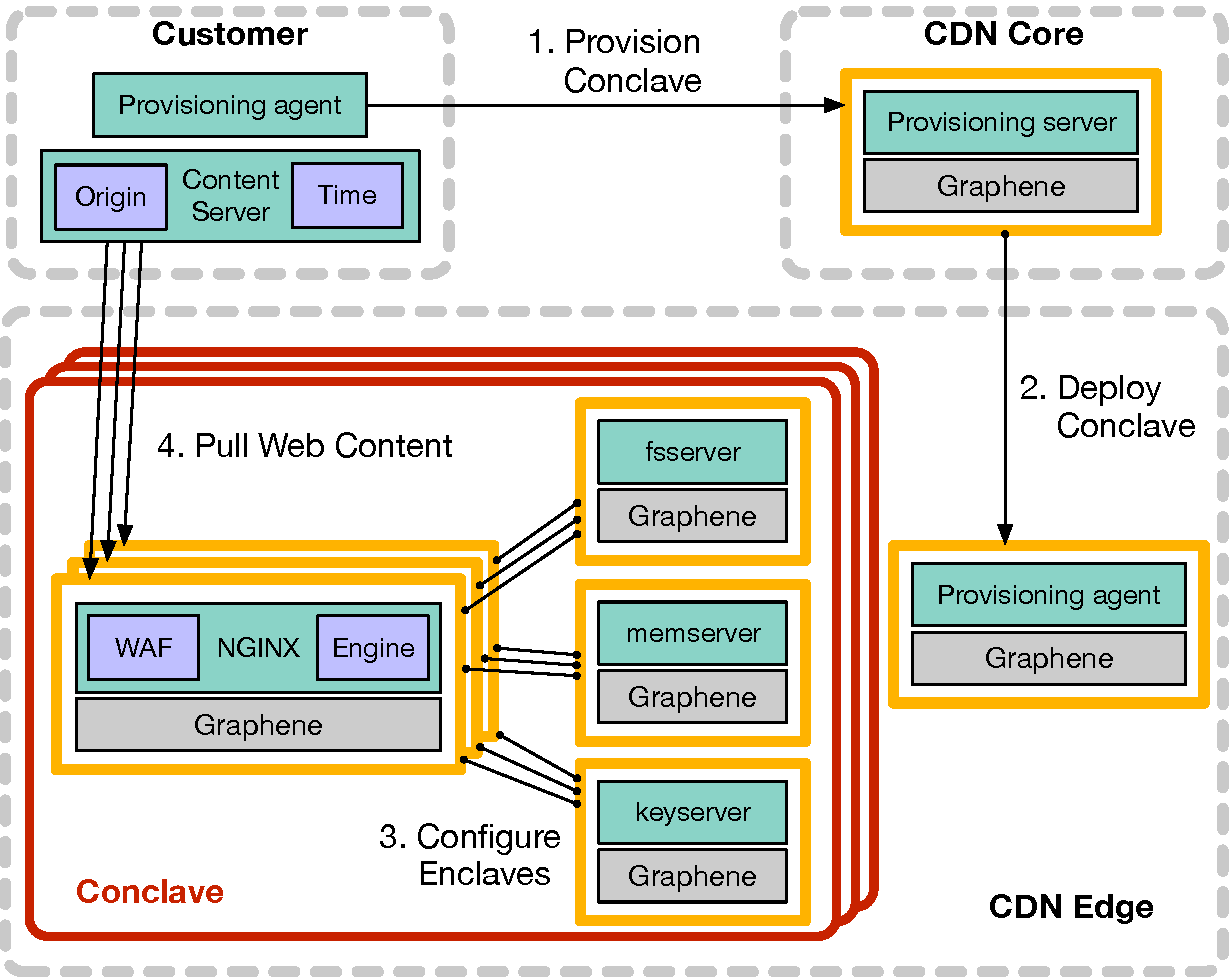
\includegraphics[width=0.48\textwidth]{figs/phoenix-design}
	\caption{Architectural design of \name. Multiple enclaves (yellow
	boxes) reside in a logical conclave (red boxes), permitting
	multiple processes and multi-tenant deployments. The CDN Edge and
	Core servers run on untrusted hosts.}
\label{fig:design}
\end{figure}

% }}}

The conclave design extends the open-source Graphene SGX libOS~\cite{graphene}
to support shared state abstractions among multiple processes.
%
Graphene~\cite{graphene} supports the critical system calls
\texttt{fork} and \texttt{exec} by automatically spawning a brand new
enclave, and performing a checkpoint-and-migration (essentially copying
the first enclave's memory pages into the second).
%
Graphene further offers some support for these separate processes
(enclaves) to communicate with one another over pipes, and implements
copy-on-write fork, signals, semaphores, message queues, and exit
notifications as RPCs over these pipes.
%
In other words, Graphene essentially turns a traditional multi-process
application into a ``distributed system'' of enclaves, along with some
basic plumbing to allow them to communicate with one another.


%% Key design challenges for libOSes include support for \texttt{fork} and
%% \texttt{exec}, and the subsequent management of shared state among the
%% processes.
%% %
%% Of the SGX-based libOSes, only Graphene supports forking, which it models as a
%% checkpoint and restore process migration.
%% %
%% In Graphene, multiple libOS instances coordinate over pipes to implement a
%% consistent, distributed POSIX abstraction, yet appear to the application as a
%% single, shared OS\@.  
%% %
%% In particular, Graphene implements copy-on-write fork, signals, semaphores,
%% message queues, and exit notifications as remote procedure calls (RPCs) over
%% these pipes.

However, two important multi-process abstractions that Graphene does not support with
confidentiality and integrity guarantees are a read-write filesystem, and
shared memory.
%
Graphene's sole filesystem, \texttt{chrootfs}, is modeled as a restricted view
of the host's filesystem.
%
%The contents of the filesystem are in plaintext; for read-only files, Graphene
%ensures the integrity of the file's contents by loading cryptographic hashes
%of the content into the enclaved libOS and verifying these hashes upon file
%reads; writable files have no integrity protections.
%
Graphene does not support shared memory at all (neither anonymous nor
file-backed).


Conclaves extend upon this prior design by leaning into the distributed
system nature of it.
%
We implement kernel services as \emph{kernel servers}; applications
act as clients, connecting to and issuing requests to kernel
services---via pipes or TLS network connections.
%
The kernel servers also run atop the libOS.
%
Our design is effectively that of a multi-server microkernel system,
similar to GNU Hurd or Mach-US, in which shared resource abstractions
are implemented as a set of enclaved daemons shared by all processes in
the system.
%% The daemons themselves also run atop the libOS\@.


\subsubsection{Conclave Kernel Servers}

Using the NGINX web server as a guide (as software representative of a
CDN edge server), we identified five key shared resources: files,
shared memory, locks/semaphores, cryptographic keys, and time.  
%
For flexibility in deployment configurations, we implement four servers
to manage these resources\footnote{Due to the common pattern of using
locks with shared memory, the memserver manages both.}:
%
We implement the fsserver, memserver, and keyserver as single-threaded,
single-process, event-driven servers that communicate with the application's
Graphene instances over a TLS-encrypted stream channel. 
%
The timeserver uses a datagram channel.
%
Each server is independent.


\parhead{fsserver}
%
For our file server, \emph{nextfs}, we extend lwext4's~\cite{lwext4} userspace
implementation of an ext2 filesystem into a networked server.
%
nextfs uses an untrusted host file as the backing store, similar to a block
device.
%
We develop three variants of this device to accommodate different security
postures, and a fourth for comparison purposes.

\vspace*{-0.5\baselineskip}
\begin{widelist}

\item 
%
\textbf{bd-std} stores data blocks in plaintext, without integrity
guarantees. This serves as a baseline in our evaluation.


\item
%
\textbf{bd-crypt} encrypts each block using AES-256 in XTS mode, the de
	facto standard for full-disk encryption~\cite{xts-ieee,xts-nist}.
%
We base each block's initialization vector on the block's ID.
%
This, too, lacks integrity guarantees, and is thus suitable only for an
	honest-but-curious attacker.


\item
%
\textbf{bd-vericrypt} adds integrity guarantees to bd-crypt, thus
	providing authenticated encryption.  It does so by maintaining a
	Merkle tree over the blocks: a leaf of the tree is an HMAC of the
	associated (encrypted) block, and an internal node the HMAC of its
	two children.
%
To keep the memory needs of the enclave small, bd-verity consults a
	serialized representation of the tree in a separate file, rather
	than use an in-memory representation.
%
The root of the Merkle tree exists both on the file and in enclave
	memory; the HMAC key exists only in enclave memory.
%
As an optimization for reducing reads and writes to the Merkle tree
	file, bd-verity maintains an in-enclave LRU-cache of the tree
	nodes.
	%
	bd-vericrypt is the appropriate choice in a Byzantine threat model.
	

\end{widelist}


\parhead{memserver}
%
We implement shared memory as filesystems that implement a
reduced set of the filesystem API\footnote{Graphene does not have a
unified filesystem and memory subsystem, and
thus \texttt{munmap} is not currently available as a filesystem operation.
}:
\texttt{open}, \texttt{close}, \texttt{mmap}, and \texttt{advlock}
(\texttt{advlock} handles both advisory locking and unlocking).
%
In our shared memory filesystems, files are called \emph{memory files}, and
either represent a pure, content-less lock, or a lock with an associated
shared memory segment.
% 
Memory files are non-persistent: they are created on the first open and
destroyed when no process holds a descriptor to the file and no process has the
associated memory segment mapped.


We implement three versions of shared memory.
%
Each stores a canonical replica of the shared memory at a known
location (either a particular server or file).
%% Each uses a scheme whereby a canonical replica of the shared memory is
%% stored at a known location.  
%
Upon locking a file, the client ``downloads" the canonical replica and updates
its internal memory maps.
%
On unlock, the client copies its replica to the canonical.
%
%Note that SGX does not provides a means for us to interpose on page accesses
%(as a page table handler would in normal Linux), and thus we must 
%interpose through the locking and unlocking system calls.
%\begin{widelist}

\vspace*{-0.5\baselineskip}
\begin{widelist}

\item 
%
\textbf{sm-vericrypt-basic} uses an enclaved server to keep the canonical
memory files in an in-enclave red-black tree.

\item 
% 
\textbf{sm-vericrypt} implements a memory file as two untrusted host files: a
mandatory lock file, and an optional segment file.
%
When a client opens a memory file, the sm-vericrypt server creates the lock file on the
untrusted host, and the Graphene client maps (\texttt{MAP\_FILE|MAP\_SHARED})
the lock file into untrusted memory.
%
The client then constructs a ticketlock structure over this untrusted shared
memory.
%
Since the untrusted host may manipulate the ticketlock's turn value, a
shadowed, trusted turn number is maintained by the enclaved sm-vericrypt
server.
%
After the client has acquired the lock, the client makes an RPC to the
server to verify the turn number.
%
The server thus acts as a trusted monitor of the untrusted monotonic
	counter.
%% As such, the server acts as a trusted, monotonic counter that monitors an
%% untrusted monotonic counter.


If a client \texttt{mmap}s the memory file, the server creates the
associated segment file on the untrusted host.
%
When the client subsequently locks the file, the client makes a \texttt{lock}
RPC to server, which returns the keying and MAC tag information for
the segment.
%
The client copies the untrusted memory segment into the enclave, and uses
AES-256-GCM to decrypt and authenticate the data.
% 
When a client unlocks the file, the client generates a new IV, copies an
encrypted version of its in-enclave memory segment into the untrusted
segment file, and makes an \texttt{unlock} RPC to the server, passing along
the new IV and MAC tag.

% \clg{I think this section can be compressed}

\item 
%    
\textbf{sm-crypt} 
	%is like sm-vericrypt, but 
	assumes the untrusted host does not
tamper with data.  As such, sm-crypt uses AES-256-CTR instead of AES-256-GCM,
and does not need an enclaved server to monitor the integrity of the ticketlock
and IV.

\end{widelist}




\parhead{keyserver}
%
The keyserver is an SGX enclave rendition of a hardware-security module
(HSM): the keyserver stores private keys and performs any private key
cryptographic operations.
%
Like Keyless SSL~\cite{keyless-ssl}, this not only maintains the
confidentiality of the private key with respect to an untrusted host,
but also isolates the key to an address space distinct from the
application's, thereby guarding against critical memory disclosure
vulnerabilities, such as Heartbleed~\cite{heartbleed-cve}.


We implement the keyserver as two components: the keyserver proper, and an
OpenSSL engine (``engine'' in Figure~\ref{fig:design}) that the application
loads as a shared library; the engine proxies private key operations to the
keyserver.
%
Unlike the fsserver and memserver clients, the key client operates at
the application layer, outside of Graphene.


OpenSSL's engine API requires the caller (in our case, NGINX) to provide an
\texttt{RSA} object, which contains the secret key.
%
To avoid having to expose the key, we modified OpenSSL to populate
\texttt{RSA} objects with dummy keys that instead serve as identifiers
that the keyserver uses to look up the real keys it stores securely.


To reduce the number of connections and avoid a dependency on the memserver for
lock files, our engine maintains the property that all keys for the same
keyserver, within the same process, share a single connection.
%
This requires that the engine detect forking by the application, which we
achieve by also associating process IDs with the \texttt{RSA} objects.


\parhead{timeserver}
%
Given that the components of a conclave must authenticate one another,
we need trusted time to guard against attacks that 
% manipulate the conclave's sense of time to
trick the conclave into accepting expired certificates.
%% (and therefore possibly
%% cracked) certificates.
%
Unfortunately, SGX itself does not provide trusted time.  
%
Its SDK~\cite{sgx-linux-sdk} provides features~\cite{sgx-trusted-time}
for retrieving coarse-grained, monotonic time through a protected clock
provided by Intel's Converged Security and Management Engine (CSME),
but not all processors support it~\cite{ayeks-sgx-hardware}.
%

%% Techniques that base wall-clock time on the \texttt{RDTSC} family of x86
%% instructions cause a \texttt{\#UD} fault in SGXv1, while in SGXv2 the
%% instruction may be modified by a hypervisor.
%% %
%% Intel's SGX SDK~\cite{sgx-linux-sdk} does provide
%% features~\cite{sgx-trusted-time} for retrieval of coarse grained, monotonic
%% time, through a protected clock provided by Intel's Converged Security and
%% Management Engine (CSME)\@.  
%% %
%% However, this feature relies on the presence of the CSME (not all processors
%% include this firmware~\cite{ayeks-sgx-hardware}), and moreover relies on an
%% enclave to securely obtain a base wall-clock time from a remote, trusted,
%% server.


Instead of relying on the CSME, we simply design a remote, signed
timestamping server.
%
The timestamping server runs outside of an enclave, on a remote trusted
machine (e.g., at the CDN's customer).
%
The timeserver's purpose is not to provide fine grained precision to
the conclaved processes, but rather to serve as an integrity check of
the time those processes receive from the untrusted host.

We modify the Graphene system call handlers for \texttt{getttimeofday},
\texttt{time}, and \texttt{clock\_gettime} to optionally proxy application
calls to a remote, trusted, timestamp signing server.
%
The use of such a timeserver, and the related parameters, such as the
timeserver's public key, are specified by the Graphene user (here, the content
provider), and hard-coded into Graphene's configuration.
%
As a freshness guarantee, each request includes a new, random
nonce, generated by the Graphene system call handlers.
%
The timeserver, in turn, returns an RSA signature over a message
consisting of the current time concatenated with this nonce.


%% As time-related system calls occur frequently in event-driven applications like
%% web servers, and as each timeserver request incurs latency due to both the
%% network and RSA operations, the Graphene client makes remote requests for  $p$
%% percent of the time-related system calls, where $p$ is a configurable
%% parameter.
%% %
%% Upon verifying a timeserver response, the Graphene client retrieves the time
%% as reported by the untrusted host, and verifies that the time the host
%% returns is within a configurable tolerance to the timeserver's time.
%% %
%% For a time-related call in which the Graphene client does not consult the
%% timeserver, Graphene checks that the time returned by the untrusted host is
%% greater than the last time value retrieved.


Our timeserver approach resembles Google's roughtime protocol~\cite{roughtime};
future work would fully port the roughtime protocol to Graphene to reduce the
need for a trusted timeserver by instead tolerating some fraction of
misbehaving servers.
%
Note, however, that, in the SGX setting, both our approach and roughtime are best
efforts; an untrusted host that identifies the traffic between the Graphene
client and timeserver could, for instance, ``slow down" time by delaying the
responses.



\subsubsection{Conclave Images} % {{{

Conclaves bundle the SGX microkernel runtime and application suite into a
deployable and executable image, reminiscent of a traditional container image.
%
When the conclave is executed, the first enclave process that is
executed is an init process, which executes the kernel servers and the
specified application proper.
%
From that point, the application can fork, spin up new applications,
and so on.


\subsubsection{Bootstrapping Trust} % {{{

%% Before we address provisioning secrets to the running conclave, we describe

We first address how the conclave, viewed as a distributed system,
establishes the trust of each member node, whether kernel server or
application process.
%
This is a chicken-and-egg problem of establishing a secure channel
between two nodes without first provisioning these nodes with, say,
private keys and certificates for mutual authentication.
%
%% 
%% 
%% %
%% There are two cases we must address: (1)~trust between a parent-child
%% relation (for instance, between the init and the processes it spawns),
%% and (2)~trust between non parent-child process relationships (such as
%% between the application nodes and the kernel servers).
%% %
%% In both cases, the problem boils down to a chicken-and-egg dilemma of
%% establishing a secure channel between two nodes without first
%% provisioning those nodes with, for instance, private keys and
%% certificates for mutual authentication.
%% %
%% If we can establish such a channel, then provisioning becomes
%% straightforward: NGINX servers can simply (and safely) read sensitive
%% key material from keyservers, and read and write sensitive user data in
%% the fsserver and memserver.



The standard approach for establishing a secure channel in an SGX setting is to use SGX
as a root of trust and enclave attestation as a form of authenticated identity,
and to merge this form of attestation into the establishment of the shared
channel secret.
%
To that end, \name follows closely from the work of Knauth et
al.~\cite{DBLP:journals/corr/abs-1801-05863}, which 
integrates attestations with TLS by adding the SGX quote as an X.509
certificate extension.
%
This has the effect of making channel establishment and SGX attestation
occur together,
atomically, with respect to the channel protocol.
%
%% prevents
%% man-in-the-middle attacks by making channel establishment and SGX
%% attestation occur together, atomically, with respect to the channel
%% protocol.
%% %
%% The core problem they address is that, to prevent
%% man-in-the-middle attacks, secure channel establishment and SGX attestation
%% must occur together, atomically, with respect to the channel protocol.
%% %
%% In order to do this, they integrate attestation with TLS by adding the SGX
%% quote as an X.509 certificate extension.
%% %
Certificate validation can thus be extended to examine these new extensions.


Adding new certificate extensions, of course, is not the full story.
%
In this setup, the enclave generates an ephemeral key pair.
%
SGX quotes are, mandatorily, over the enclave image, the enclave signer,
non-measurable state, such as the enclave mode (e.g., debug vs production),
and, optionally, any additional data (user data) the enclave wants to
associate with itself.  
%
The trick for ensuring the atomicity of attestation and secure channel
establishment is for the enclave to specify as user data a hash of the ephemeral
public key.
%
Since the key pair is created within the enclave, and since only an enclave can
get a valid quote, such user data binds the key pair to the enclave.
%
The enclave then generates a self-signed certificate for this ephemeral public
key, which includes the aforementioned extensions for the quote and IAS
verification.


In our conclave setup, the attestation is a local attestation, and validation of
the quote is based on a list of valid attestation values in the manifest.
%
Specifically, the manifest specifies a graph of which processes can establish
secure channels with one another.


\subsection{Evaluation}

Figure~\ref{fig:macrobench-single-tenant-lat-throughput} shows
request latency and throughput results for the four configurations.
%
Due to the RSA private key operation in the TLS handshake, Linux becomes
CPU-bound at four workers (our test machine has four physical cores) and
saturates the Ethernet link for tests with a 100~KiB payload and more than one
NGINX worker.
%
Linux-keyless shows that the concurrency of the keyserver levels
off with two workers, and thus that the two NGINX worker configuration of
Linux-keyless is an upper-bound on the performance we can hope to achieve
with the other conclave configurations.
%
%In addition, whereas Graphene-crypt shows increased performance as the number
%of workers increases, Graphene-vericrypt tops off at two workers, before
%showing worse performance with more NGINX workers.
%
To compete with a one worker Linux configuration, Linux-keyless needs two
workers, and Graphene-crypt needs four; Linux with two or more workers beats
all conclave configurations.


\begin{figure}[t]
	\centering
    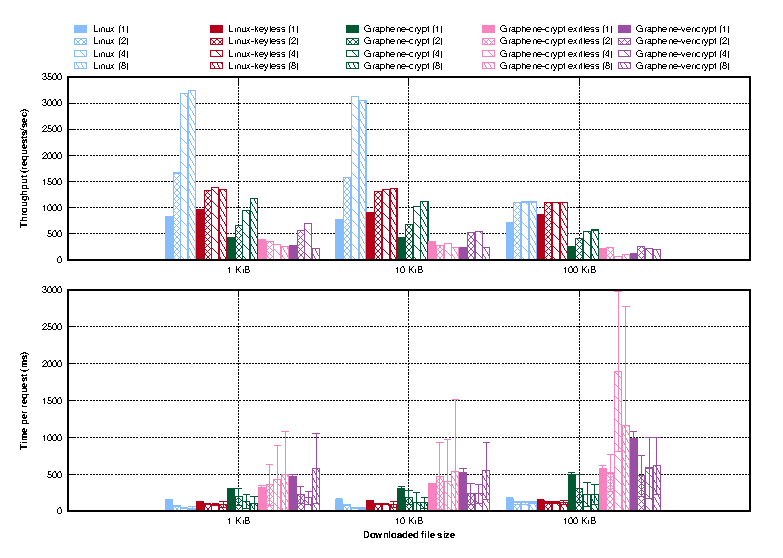
\includegraphics[width=0.5\textwidth]{figs/macrobench-single-tenant-lat-throughput}
	%
	\caption{Throughput and latency for single tenant configurations.
    The legend indicates the number of NGINX worker processes.
    We include the standard deviation of the latencies as error bars.}
	%
	\vspace*{-4pt}
    \label{fig:macrobench-single-tenant-lat-throughput}
\end{figure}

\section{Codomains Introduction}
\label{sec:codomains-intro}

A cooperative domain, or \emph{codomain}, is an isolation domain
that a thread may migrate to over the course of its evolution, such as another
process, another host, or an SGX hardware enclave.
%
I explore system primitives for using codomains that enable a developer to
write a monolithic program that executes over multiple domains, with the
underlying system being responsible for moving the execution between domains,
maintaining resource consistency across domains, and restricting
information flow among domains.
%
The application need not directly construct codomains; a monitor or emulator
could do so on the process's behalf, thereby enabling opportunities for
instrumenting existing, legacy, applications.
%
In contrast to prior work in program partitioning, codomains present
a language-neutral, run-time mechanism for switching domains, rather than
resorting to language-specific or compile-time techniques.


\parhead{Codomains vs. Conclaves}
%
Codomains are orthogonal to conclaves, though the implementation may
use conclaves to support SGX domains.
%
Codomains further differ from conclaves with respect to use cases, and the
method for constructing trust boundaries.
%
Whereas conclaves are a solution for preserving the confidentiality of a single
\footnote{
Conclaves may comprise
multiple parties, but these parties must trust one another (or, as in
the case of NGINX multiplexing multiple parties, NGINX must be trusted
to isolate one party's components from another).
}
party's data when running an application on an untrusted cloud,
%
codomains can further express solutions for multi-party and
federated computations.
%
With conclaves, a deployer statically specifies the trust boundaries based on
which components (processes) may communicate with one another;
%
%Boundaries are binary; trust means unfettered communcation; no trust means no
%communication.
%
with codomains, the boundaries themselves may change over
the application's evolution, and data, rather than code, may drive the boundary
construction.
%
Finally, whereas conclaves take an approach of hoisting the entire application
into enclaves, codomains use enclaves in an on-demand, as needed, fashion.

%\section{Codomains Background}
\label{sec:codomains-background}

We focus on two use cases that involve multiple parties cooperatively running
an application where the input of at least one party is confidential:
(1) outsourcing TLS-based applications to a third party, and (2) federated
analysis over private data.


\parhead{Outsourcing TLS applications}
%
In this setup, a company uses a third party, such as a cloud host or cloud
service, to operate an application server, such as for web, DNS, or mail.
%
Operationally, the status quo is for the company to shares or otherwise entrust
the third party with the application's private keys.
%
This has significant implications on the trust model of the PKI and the web
writ large, as these third parties can arbitrarily impersonate any of their
customer organizations.
%
Our goal is to design system primitives that allow developers to write or
patch, and deployers to configure, such applications with the property that the
company retains exclusive custody of its private keys.


\parhead{Collaborative Data Processing}
%
In this setup,  the aggregate dataset consists of the confidential, local,
datasets of multiple parties.
% 
The parties themselves might be mutually distrustful, or may simply be
prevented by law from sharing their data.
%
An analyst wants to process the datasets to determine some non-confidential
result.
%
With federated databases, the result may be the cardinality of an intersection
across the datasets.
%
With federated learning, the result may be the global model parameters (such
as the weights of a deep neural network), derived from the aggregation of the
parameters from each party's locally-trained model.
%
Our goal is to enable the developer to express, in a
single program, the multi-party nature of the application, with the underlying
system managing the application's distribution across parties. 


While our system will present an interface for partitioning the application
across the parties, partitionioning alone does not prevent private data
leakage.
%
For instance, local results and parameters may, by themselves, reveal
information about the private data samples.
%
Thus, orthogonal to our system, the application may additionally require
methods for achieving differential privacy, such as by adding a carefully
chosen amount of noise to the local results.


\subsection{Threat Model}

We assume an honest but curious (HbC) threat model: each party faithfully
executes the program, but may analyze their portion of the execution to try to
recover the private data of other principals.
%
We assume that the parties trust the application; that is, the application does
not deviate abitrarily from its stated purpose, and does not actively try to
leak sensitve data.
%
We assume that the application is bug-free, and thus our model omits external
actors, such as a remote attacker.


An HbC model is not inherent, but is reasonable for our use cases,
given the mutually beneficial incentives among the parties, and further
simplifies the system design.
%
Consider, in contrast, a more adversarial model where the parties, or the
application itself, may abuse the interface for domain switching---as by
switching at an unexpected state, or switching to a malicious code page---for
the purpose of actively leaking sensitive data. 
%
In this model, the target domains must first, externally, validate the
execution state against an expected starting condition before commencing
execution.


An interesting design point related to the threat model is whether the
application is globally public, or whether some portions are private and thus
confidential to a party. 
%
For instance, in the scenario of a company outsourcing a web server to a CDN,
the CDN's web server may be proprietary, and the CDN operator in turn may be
unwilling to allow the server's execution to switch to a company's domain
for fear of leaking proprietary knowledge.
%
Naively, this scenario reduces to specifying that private code pages should be
pinned to the owning domain, and that execution may switch domains only at
non-private points in the application's execution.
%
The tricky aspect is that the data written by private code pages should,
likewise, be private, as sharing such data pages could reveal aspects of
the private code.
%
We consider this feature as future work, but briefly revisit the idea in
\S\ref{sec:codomains-challenges}.


Typical of other work in this area, we consider side-channels out of scope.


%Within the realm of secure, federated data processing, the need for differential
%privacy is virtually unavoidable, as local results and parameters may, by
%themselves, leak information about the underlying data samples.
%%
%Differential privacy (DP) is a property of randomized queries that take a
%database as input and return a statistical result, such as an aggregate.
%%
%The database is a collection of rows, with each row containing data
%from one individual.
%%
%Informally, queries are differentially private if arbitrary changes to a single
%individual’s row result in only statistically insignificant changes in the
%function’s output distribution. 
%%
%Thus, the presence or absence of any individual has a statistically negligible
%effect.
%%
%Practical solutions for achieving DP typically rely on adding a carefully
%chosen amount of noise to the result.
%%
%DP offers a provable bound on the amount of information that an adversary can
%learn about any individual, even with access to auxiliary information


% DP Definition
%
%Differential privacy (DP): by
%disallowing certain qeuries and carefully adding a chosen amount of noise to
%the result of others, it is possible to give a strong upper bound on how mcuh
%an adversary could learn about an invididual person's data.
%


% such as an aggregate statistical value, or to learn the parameters to
%a machine learning model trained across the datasets.


%%%% FEDERATED LEARNING
%
%Federated Learning (FL) trains an algorithm across
%multiple principals holding local, confidential, data samples, thereby allowing
%the principals to build a common machine learning model withouth
%sharing their data.
%%
%%
%As local parameters may, by themselves, leak information about the underlying
%datasamples, FL may further incorporate DP or secure aggregation.


%DStress is a system that can efficiently perform computations on graphs taht
%contain confidential data. Dstress assumes that the graph is physically
%distributed across many participants, and that each participaint only knows a
%small subgraph; it protects privacy by enforcing tight, provable limits on how
%much each participant can learn about the rest of the graph.
%
%The motivating usefaul is measuring systemic risk in financial networks. The
%requried information is extrmeemly sensisive because it directly reflects the
%business strategy of each bank.
%
%It is well known taht many interesting thnigs can be learned by collecting and
%analyzing large graphs. Tools assume that the user has a property Graphen G
%(that is, a graph that has some data asscoiated with its vertixes and/or edges)
%and wishes to compute com function F(G) over this graph and itsp roperites.
%
%However, there is another class of use cases where the graph G contians
%sensitvie information and is spread across multiple administratigve daomins. In
%this situation, each domain knows only a subset of the vertexes and edges, so
%it cannot compute F(G) on its own, but the domains may not be willing to share
%their data with each other because of privacy concerns.
%
%
%DStress support vertex programs; it addresses the first challenge with a
%special graph-computation runtime tha can execute vertex programs in a
%distributed fashion, using MPC and a varint of ElGamal encryption
%(homomorphic for transferring data between domains, and it addresses the
%second challenge by keeping intermediate results encrypted at all times, nad by
%offering differential privacy on the final result.
%
%Our approach is based on two key insights. Our first observation is that much
%of the enormous cost of the MPC-based strawman comes from the fact that the
%graph is itself confidential and therefore must be an input to the computation.
%We can get around this by fomrulating the funciton F as a vertex program – that
%is, as a sequence of comptuations at each vertex that are interlevaed with
%message exchagnes over the edges – and by executing it in a distributed
%fashion. The main challenge is to prevent information leackage thorugh
%intermediate results. In DStress, we asccomplish this with a combination of
%secret sharing, small MPC invocations for the computations at each vertex, and a
%special protocol for transferring shares without revelaing the topology of the
%graph. our second key insight is that we can use differential privacy to
%achieve output privacy.



\section{Codomains Design}
\label{sec:codomains-design}

In this section, I explore the concept of codomains to arrive at an
API for developing programs for such an execution model.
%
The core features I need are pinning data to a domain and switching
(migrating) between domains, while the core challenges I face are providing
resource consistency and mechanism transparency.
%
I first introduce a building-block abstraction called coprocesses, and then
describe how I implement codomains on top of coprocesses.
%
I then discuss techniques for \emph{backfitting} codomains, at run-time, onto legacy
application binaries by means of running the application on a
taint-tracking-enhanced emulator.
%
Under this scheme, a user specifies a data policy that defines the domains and
their access privileges to the various application data, and the emulator
handles switching domains on data access based on these privileges.
%
I conclude with challenges that I anticipate when implementating codomains and
applying them to applications.


\subsection{Coprocesses}

%% definition
A \emph{coprocess} is a process to which a client process yields its
execution.
%
My interest with coprocesses is handling, in userspace, services requisite to
codomains: distributed shared memory, distributed fileystems, and the
checkpointing and restoring of the client process, while further enabling both
explicit and implicit yields to these services.
%
In these respects, a coprocess is similar to a library operating system, but
one that operates in an address space distinct from its client process: instead of
trapping directly to the kernel, the process traps to its coprocess, which may
either service the trap on its own, or forward the trap to the kernel.

%% TODO: sentence about why in userspace, or some tie-in to exokernels

%% suggest that the concept exists in narrow forms.
Coprocesses are not a novel idea: operating systems already partially expose the
concept through system calls like \texttt{ptrace} and
\texttt{userfaultfd}, which allow one process to control aspects of another,
and through runtime loading techniques such as \texttt{LD\_PRELOAD}, which
enable shims for proxying a process's library calls.
%
Part of my work is in exploring whether these existing facilities are
sufficient for my flavor of coprocesses, or whether I must develop additional
system calls for that purpose.


\parhead{Coprocess API}
%% Becoming a coprocess; attaching to
%
In Listing~\ref{lst:coproc-api}, I present the coprocess API\@.
%
The API design presents the coprocess as an ambient service to the process
(similar to the kernel), abstracting away any details of IPC between the
coprocess and process.
%
A process becomes a coprocess by calling \texttt{coproc\_create}, whose
argument is a unique pathname identifying the coprocess, and whose return value
is a socket-like descriptor for communicating with future client processes.
%
A client process attaches to a coprocess by calling \texttt{coproc\_set}, passing as an
argument the path representing the coprocess.
%
Analogous to how calling \texttt{accept} on a listening socket returns an
active client socket, calling \texttt{accept} on the coprocess's descriptor
returns a \emph{process decriptor} for an attaching process.
%
A process may have at most one coprocess, and a coprocess may service multiple
processes.
%
%A processes's coprocess, and the state of being a coprocess, are attributes
%within a process's control block.


%% Interaction between a process and coprocess
A process synchronously interacts with its coprocess through
\texttt{coproc\_call}; \texttt{coproc\_call} is to a coprocess as a system call
is to the kernel, and developers may implement application-specific messages
on top of this call.
%
A process may also synchronously invoke its coprocess through
\texttt{coproc\_raise}.
%
The semantic difference between \texttt{coproc\_raise} and
\texttt{coproc\_call} is that \texttt{coproc\_raise} does not return---the
process does not receive a return value and does not expect to resume
execution at the instruction following the call to \texttt{coproc\_raise}.
%
In these respects, \texttt{coproc\_raise} is analogous to the process raising
an exception.

\begin{lstlisting}[
    frame=single, 
    caption={Coprocess API},
    captionpos=b,
    label={lst:coproc-api},
]
int coproc_create(const char *path)
int coproc_set(const char *path)
int coproc_call(int msgtype, void *args, void *result)
void coproc_raise(void *args)
\end{lstlisting}


%\parhead{Coprocess Events}
%
% TODO: whereas the coprocess API section describes the interface mostly
% from the process's perspective, now describe the types of messages a
% coprocess reads throught the socket decriptor thtat coproc_create returned.


\parhead{Coprocess Server}
% TODO: define and \emph{} coprocess server, since we use that term later with
% codomain.
%
Before delving into codomains, consider how switching execution between domains
would appear at the coprocess-level.
%
A process in domain A sets a coprocess and yields execution.
%
The coprocess checkpoints the process's thread and then makes a remote request
to a service in domain B\@.
%
B's service may either be a coprocess, or a service that executes a new
coprocess---a \emph{coprocess server}.
%
Regardless, the service must also execute a stub program that first attaches to
the coprocess and then launches a loader that restores A's thread.
%
Any page faults during the restoration process trap to the coprocess on B,
which may request the page from the coprocess on A.


\subsection{Codomains}

I first introduce codomains programmatically with a two-party example in
Listing~\ref{lst:isolating-key} that isolates private key operations to a
single domain, \texttt{domain\_priv}; all other parts of the application
execute in the initial domain, \texttt{domain\_pub}.

\begin{lstlisting}[
    frame=single, 
    caption={Isolating a private key to a domain},
    captionpos=b,
    label={lst:isolating-key},
    numbers=left,
    numberstyle=\tiny,
    xleftmargin=2em,
    framexleftmargin=1.5em,
    ]
int domain_priv;
int domain_pub;
char *key;

load_key(path) {
    domain_pub = co_switch(domain_priv)
    key = read_file(path)
    co_pinmem(key)
    log(log_fd, "loading key (%s)", path)
    co_switch(domain_pub)
    return key;
}
 
sign(key, buf, buflen) {
     domain_pub = co_switch(domain_priv)
     signature = do_sign(key,buf)
     log(log_fd, "signed something");
     co_switch(domain_pub)
     return signature; 
 }

main(int argc, char *argv[]) {
    coproc_set("/srv/foo.coproc");
    domain_priv = co_attach(url, rspec)
    load_key(argv[1])
    sign(key, argv[2], strlen(argv[2]))
}
\end{lstlisting}


\texttt{domain\_pub} sets its coprocess on line 23, and then attaches to 
\texttt{domain\_priv} on line 24.
%
The \texttt{url} argument to \texttt{co\_attach} specifies the coprocess server
for \texttt{domain\_priv}, and \texttt{rspec} describes the resources (such as
filesystem, open descriptors, memory pages) that \texttt{domain\_pub} exports
to \texttt{domain\_priv}.
%
The return value of \texttt{co\_attach} is a descriptor for the attached
domain; the descriptor only has meaning to the coprocess, and is not present
in the process's kernel-level file descriptor table.


On line 25, the process calls \texttt{load\_key}, which then invokes
\texttt{co\_switch} to switch to \texttt{domain\_priv}.
%
\texttt{co\_switch} checkpoints the thread on \texttt{domain\_pub} and restores
the thread on \texttt{domain\_priv}.
%
\texttt{co\_switch} returns a descriptor representing the domain that
initiated the switch.


Within \texttt{load\_key}, \texttt{domain\_priv} pins the memory pages storing
the private key by invoking \texttt{co\_pinmem};
such pages are cloaked when executing in another
domain, and uncloaked when a thread executes in the caller's domain.
%
The \texttt{load\_key} and \texttt{sign}
functions perfectly encapsulate the key's use, and thus  \texttt{co\_switch}
simply ``wraps" their invocation.


\parhead{Codomain API}
%
In Listing~\ref{lst:codomain-api}, I present the codomain API\@.
%
Since I covered \texttt{co\_attach} and \texttt{co\_switch} in my prior
description of Listing~\ref{lst:isolating-key}, I will focus here on describing
the \texttt{co\_rspec} structure, as well as its mutators and accessors.
%
\texttt{co\_rspec} describes the resources that the calling, owner, codomain
exports to a peer codomain; when the peer accesses the resource, the peer's
coprocess either proxies the operation to the owner's coprocess, or replicates
the resource, depending on policy.
%
In the case of file resources, \texttt{rspec} essentially specifies a union
mount for the peer codomain, with some files and resources belonging to the
owner domain.
%
The \texttt{rspec} parameter of \texttt{co\_attach} specifies the initial
export policy; \texttt{co\_getrspec} may latter refine this policy (where
the \texttt{fd} parameter is the descriptor for the peer codomain).


I implement the API entirely on top of the coprocess API of
Listing~\ref{lst:coproc-api}; in particular, \texttt{co\_attach},
\texttt{co\_getrspec} and \texttt{co\_setrspec} invoke \texttt{coproc\_call},
and \texttt{co\_switch} invokes \texttt{coproc\_raise}.
%
Auxiliary functions like \texttt{co\_pinmem} (used in
Listing~\ref{lst:isolating-key}), and analogous functions for pinning other
resource types, are implemented on top of \texttt{co\_setrspec}.

% XXX: compare to 9p protocol: http://man.cat-v.org/plan_9/5/intro
\begin{lstlisting}[
    frame=single,
    caption={Codomain API},
    captionpos=b,
    label={lst:codomain-api},
]
int co_attach(char *url, struct co_rspec *rspec)
int co_switch(int fd)
int co_getrspec(int fd, struct co_rspec *rspec)
int co_setrspec(int fd, struct co_rspec *rspec)
\end{lstlisting}

% TODO: describe rspec further
%\begin{lstlisting}[
%    frame=single,
%    caption={Codomain API},
%    captionpos=b,
%    label={lst:rspec},
%]
%struct co_rspec {
%    TODO
%};
%\end{lstlisting}
%

%%
%In the \texttt{load\_key} function of Listing~\ref{lst:isolating-key}, the
%application calls \texttt{read\_file} on line 7,
%which opens a file, reads in the contents, and then closes the file.
%%
%Suppose \texttt{domain\_pub} first tested if \texttt{path} existed;
%would that test succeed?  
%%
%Beyond this simple example, suppose that \texttt{domain\_priv} created a
%file; would \texttt{domain\_pub} be able to view it? 
%%
%
%% XXX: you need the process on B to call co_setrspec() before execve() to
%% specify the resources.
%
%%
%%In Listing~\ref{lst:isolating-key}, the domains do not need to share the filesystem:
%%\texttt{domain\_pub} and \texttt{domain\_priv} have completely separate
%%filesystems, and path names may even clash between the two.
%
%
%Similar issues exist for file descriptors.
%%
%For instance, in the example, \texttt{log} writes the log statements to a log
%descriptor.
%%
%This descriptor could represent a terminal, a file, or a socket.
%%
%We may want the write to proxy the call back to \texttt{domain\_pub} (which
%would be necessary in the socket case), or to perform the write locally, as by
%``migrating" the underlying resource from \texttt{domain\_pub} to
%\texttt{domain\_priv} (which may be more appropriate for the terminal case).
%%
%In other words, \texttt{rspec} not only needs to say which resources
%are shared, but also how they are shared.
%


\parhead{Distributed Shared and Cloaked Memory}
%
%% why codomains need DSM
For multi-threaded and multi-process applications, I must consider how the
system maintains consistency of memory layout and coherency of shared memory
among threads operating concurrently on multiple codomains.
%
This problem generally necessitates some form of distributed shared memory.


%% DSM definition and how DSM fits into codomain design
% TODO: cite for DSM protocol papers
\emph{Distributed shared memory} (DSM) provides distributed processes with a
shared address space accessible through the conventional memory access protocols
(in contrast to message passing).
%
DSM protocols differ with regard to data granularity, synchronization,
and consistency models, though page-based granularity and \emph{sequential
consistency} are common.
%
A common paradigm is the use of write-invalidations: each domain
write-protects shared pages; when a domain tries to write to such a page, a
protection fault occurs.
%
In the case of codomains, the coprocess would notify peer domains that the
page is locked for writing, and then make the page writeable to its process.


%% codomain-specific needs/concerns wrt to DSM
In addition to normal DSM behavior, the coprocess's DSM implementation must
also handle cloaked pages.
%
When a domain accesses a cloaked page, the result is a fault to the process's
coprocess.
%
The coprocess either treats the fault as a segmentation fault (likely
terminating the process), or as a page fault.
%
In the latter case, the coprocess handles the page fault by moving execution to
the domain of the page owner, as if the application implicitly called
\texttt{co\_switch}.
%
The application dictates fault semantics via the \texttt{rspec} parameter when
attaching to the codomain.


\parhead{Checkpoint/Restore}
%
\emph{Checkpoint/restore} (C/R) is the ability to snapshot the state of an
application and then later restore it to a running state, possibly
on a different system.
%
Two conventional uses for C/R are live migration of containers,
and the incremental snapshotting of an application, as for recovery
after a crash, outage, or malware infection.
%
Several research and commercial
systems~\cite{transparent-process-migration,dmtcp,popcorn-migration} implement
C/R, but CRIU~\cite{criu}, which manages the operation from userspace, is the
\emph{de facto} standard on Linux.
%
For the purposes of querying the kernel for a process's state, and later
passing that state back to the kernel when restoring the process,
CRIU makes heavy use of the \texttt{/proc} file system, netlink sockets,
system calls, and \texttt{ptrace}, the latter of which injects parasite code
to dump any remaining information.


There are several issues with composing these existing C/R systems, and CRIU in
particular, with codomains, which reflect a mismatch in their use cases, design
decisions, and assumptions.
%
The major points of incongruity are (1) the coarse-grained C/R of a process vs.
the fine-grained C/R of a thread; (2) infrequent vs. frequent C/R operations
(and the application's associated sensitivity to the latency of the operation);
(3) the inverse nature of checkpointing with restoring vs. C/R in the presence
of cloaked data and resources; and (4) the use of C/R to move a whole system,
rather than using C/R to distribute a single system.
%
I merely bring up these issues to note that the codomain design does not
necessarily entail an implementation that bundles existing functionality, and
that an implementation might instead add kernel functionality such that the
coprocess can retrieve thread state from a process descriptor.


\parhead{Parallel Execution}
% A computational modelis a conceptual view of the types of operations availableto a program.
%
%
When developing a new distributed, or, specifically, federated, application
with codomains, it is useful to have some notion of \emph{parallel
execution}---that is, a single-instruction, multiple-data computational model.
%
In a single-process, single-host setting, pthreads are the mechanism for
parallel execution; in a distributed setting, a framework such as MPI
may be used to develop a monolithic program that then executes a parallel
computation as a distributed system.
%
I ask whether codomains compose with pthreads to achieve a distributed,
parallel programming model similar to MPI.  \footnote{A related question is
whether codomains can augment MPI; I leave this as interesting future work.
}


For such computations, maintaining the memory and fileystem consistency across
codomains may not be a concern; it may be more natural for threads running in
separate codomains to have their own private address space and file system that
a master codomain has initialized.
%
When the codomain thread exits, it merely needs to return a value to some
master codomain, rather than overlay shared pages that contain the return
value.
%
% TODO: probably add arguments to co\_switch.
%
Moreover, the return value itself might need to be sealed (encrypted) to a
particular domain, such as to an enclave domain that then securely aggregates
the return values of all the codomains.


I sketch a design for how this might work in Listing~\ref{lst:lwc-parallel}.
%
The design relies on lightweight-contexts~\cite{lwcs}, which is an
OS-abstraction that allows a process to have multiple contexts (a collection of
resources that includes an address space, credentials, and file descriptor table),
and to switch in a coroutine-like fashion between these contexts over the
process's evolution.
%

%A simple, perhaps naive approach, would be that the private domains encrpyt the
%output using the public key of the enclave's domain.
%%
%This then brings up the question of how domains know of the existence of other
%domains; in particular, must ``capabilities" for other domains be passed in the
%\texttt{rspec}.


\begin{lstlisting}[
    frame=single,
    label={lst:lwc-parallel},
    numbers=left,
    numberstyle=\tiny,
    xleftmargin=2em,
    framexleftmargin=1.5em,
    caption={Combining codomains with light-weight contexts for parallel computation},
    captionpos=b,
]
int snapfd;

thr_func(worker_fd) {
    main_fd = co_switch(domain_fd)
    val = lwcswitch(snapfd)
    co_switch(main_fd);
    return val
}

main() {
    enclave_fd = co_attach()

    snapfd = lwccreate()
    if (snapfd != -1) {
        open("data.dat");
        val = do_work()
        encrypt_to_enclave(val)
        lwcswitchdicard(val);
    } 

    for 1 to N:
        pthread_create(thr_func, worker_fd)
            
    vals  = join_all_threads()
     
    main_fd = co_switch(enclave_fd)
    sum = secure_sum(vals)
    co_switch(main_fd)
}
\end{lstlisting}


\subsection{Supporting Legacy Applications with Codomains}
\label{sec:codomains-legacy-apps}

In Listing~\ref{lst:isolating-key}, partitioning the application simply
involved wrapping functions that access private data with calls to
\texttt{co\_switch}.
%
Consider the case where a party's private data cannot be encapsulated in a
functional interface.
%
My approach is to run the process under a \emph{dynamic binary
instrumentation} (DBI) framework.
%
DBI frameworks consist of an emulator that instruments and dispatches the
application's code, allowing the emulator to regain control at the end of each
basic block\footnote{A \emph{basic block} is roughly a sequence of instructions
that terminates in a jump.}.
%
I provide instrumentation code that tracks the propagation of the sensitive
data over the course of the computation; as sensitive data taints other data,
the instrumented instructions invoke \texttt{co\_pinmem} on the associated
data's page.


With this  method, I still assume that sensitive data is programmatically
introduced (as through \texttt{struct co\_rspec}), and that a coprocess
implicitly invokes \texttt{co\_switch} when a domain faults accessing cloaked
data.
%
However, it is not entirely obvious how the process, once migrated to the data
owning domain and running under a DBI framework, safely invokes
\emph{co\_switch} to switch back to the original faulting domain.
%
In general, such migration conditions are application-specific.
%
One application could simply wait until the process similarly faults on
cloaked data; another could add instrumetation that invokes
\texttt{co\_switch} after so many instructionrs have executed sequentially over
non-sensitive; and yet another could wait for the next programmatic instance of
\texttt{co\_switch}.


Composing codomains with a taint-tracking DBI framework is potentially
beneficial in two other respects: (1) as a ``safety belt" for programs
that may inadvertently leak sensitive data, and (2) as a method for
partitioning black-box, trusted applications, that require a party's sensitive
input, such that the sensitive input does not leak to other parties.
%
With black-box partitioning, the DBI framework may have to declassify tainted
data for liveness concerns; for instanace, taint-tracking instrumention would
mark a signature as tainted, even though it is not semantically sensitive.
%
Declassificaiton requires hooking at least the epilogues of such functions.
%
In essence, this results in \emph{half-wrapping}, whereby a domain could be
migrated to at any point based on faults, but has well-defined exit points and
exit conditions.


\subsection{Enclaves as Codomains}
\label{sec:enclaves-as-codomains}

There are multiple challenges with migrating execution into an enclave; we
distill these challenges down to two problems: maintaining memory coherence
with peer codomains, and supporting dynamic attestation.


Memory coherence between a non-enclave codomain and enclave-codomain is
complicated due the differences in memory layout, specifically with regards to
the heap and thread context structures.
%
Additionally, lazy migration and DSM protocols must address the limitation that
all enclave memory must be commited at the time of enclave initialization, and
that the protection attributes of these memory pages cannot be changed during
enclave execution.
%
SGX2 overcomes some of these restrictions by permitting increased dynamic memory
management within an enclave, but at the expense of greater enclave
implementation complexity.
%
%Regardless...

With SGX, an enclave packaging step produces a measurement of the enclave image by
emulating the measurement tasks that the Intel hardware will perform when
loading the enclave.
%
With codomains, however, it is not immediately clear what parts of the
application constitute an enclave image.
%
This issue is, in part, bypassed by having the enclaved code simply be a loader
program that dynamically loads the relevant portions of the application, but
given that the executable pages could comprise only a small part of the
application, and that the initial state of the data pages is generally unknown,
it's not immediately clear what meaningful attestation the enclave could
provide to a remote party.


\subsection{Additional Challenges}
\label{sec:codomains-challenges}

\parhead{Deadlock}
%
Applications running over codomains are susceptible to a form of deadlock
whereby, during the course of a thread's execution, the thread reaches an
instruction that accesses two pieces of data, each pinned to a separate domain.
%
In some cases, this may be indicative of a programming error, as by failing to
partition the application so that the computation occurs in a secure enclave,
if available.
%
On the other hand, a plausible, inadvertent, deadlock scenario is a server that
supports multiple tenants and uses a global data structure to manage the
(pinned) keys across all tenants.
%
In such cases, the application may need to be patched to correct the offending
memory layout.
%
In the general case, the problem is one of secure multi-party computation, and
an interesting area of future work is for the system to just-in-time compile
and emit garbled circuits when it detects such events.


\parhead{Private Code}
%
In my codomain design, I focus on cloaking sensitive data, but proprietary
software also necessitates cloaking sensitive code.
%
Na\"{i}vely, this scenario reduces to pinning private code pages to the owning
domain, and restricting domain switches to non-private points in the
application's execution.
%
However, this restriction alone is insufficient, as data written by private
code pages should, likewise, be marked private, as sharing such data pages
could reveal aspects of the private code.
%
For privacy with respect to codomains, this result requires a tight coupling
between the proprietary code and its memory allocator.
%
If the application is not coducive to achieving this coupling programmatically,
then the solution may require an alternative form of taint-analysis that
additionally applies taint to instructions, and propagates taint from
instructions to operands, rather than solely propagating taint from one memory
operand to another.


\parhead{False sharing}
%
A disadvantage of the integration between virtual memory and DSM is that the
unit of access and locking are constrained to be a page.
%
If the application allocates multiple data structures on the same page, then
this constraint can lead to \emph{false sharing}, wherein distinct private data
structures appear shared due to colocation on the same page.
%
Operationally, false sharing leads to thrashing.
%
A similar phenomenon occurs when applying taint tags or otherwise pinning
memory at page granularity.


\parhead{Inadvertent data leakage}
%
Although codomains present an interface for partitioning an application across
trust boundaries, partitionioning alone does not prevent private data leakage.
%
For instance, local results and parameters from a federated learning
application may reveal information about the private data samples.
%
Thus, orthogonal to codomains, the application may additionally require
methods for achieving differential privacy, such as by adding a carefully
chosen amount of noise to the local results.


%\parhead{Integrity}
%
% TODO: quote the work that criticizes keyless-ssl as just being an encryption
% oracle.



% TODO: how is the pinned domain marked in the page table?  (a unique
% memory protection key):.
%
% TODO: what happens if pinned data is written to a descriptor/file?


% TODO: try to translate switch() into a "remote" lwc:
%  
%   fd = lwccreate(resource_spec)
%   ret = lwcswitch(fd)
%   if (parent):
%       switch
%       migrate
%   else:
%       

%   Antoher issue is that reads and writes to the file must subsequently be
%   kept in sync with any toher processes using that file on src. 
%    
% - What happens if dst tries to read/write a descriptor that was opened on src?
%
%   Similar situation where the file either needs to migrate to dst or the
%   calls proxied.
%
%   You can think of migrate() of being like a fork, and specifing which file
%   descriptors are kept open and which are closed across the join.  Or similar
%   to the mem_pin, src would pin the desripotrs, saying that access should
%   either fault, migrate back, or be proxied.
%
%   For the crypto and federated examples, there's no need for sharing
%   filedescriptors and files.
% 
%   - suppose domian_priv forgot to close the file descriptor as part of
%     read_file -- would that descriptor then be open in domain_priv?

\section{Codomains Evaluation}
\label{sec:codomains-eval}


\subsection{Macro-benchmarks}

\parhead{Webserver}
%
I evalute the request throughput and latency of a webserver, such as NGINX,
running in a standard Linux environment, and compare against a configuration of
the webserver running with codomains, where a separate domain isolates each
website's private TLS key.
%
I also compare the codomain version of the webserver to 
static partitioning schemes~\cite{eleos,glamdring,privtrans} that achieve
the same isolation.
%
When comparing to static partitioning schemes, I am interested not only in the
performance differences, but also how the the boundaries determined by each
scheme differ.
%
The benchmark affords multiple variants, such as investigating how codomains
scale with multiple tenants (multiple websites multiplexed by the same
webserver), how the system performs when the webserver itself contains
private data that must be cloaked from tenants, how well different server
models (such as multi-process vs. multi-threaded) interact with codomains, and
how host-codomains compare to enclave-codomains.


\parhead{Federated Data Analysis}


\parhead{Federated Learning}


\subsection{Micro-benchmarks}

With the micro-benchmarks, I am interested in isolating the cost of each
facet of codomains---thread migration, taint tracking, the DSM protocol.
%
For such purposes, I envision developing a small set of multi-party programs
drawn from the literature, such as:

\begin{widelist}
\item \textbf{Timestamp signing server:} Returns a signature over the current
time to each client; I assume the server's key must be isolated from the
server's host.
%
\item \textbf{Richest protocol:} Computes the richest principal.
%
\item \textbf{GPS protocol:} For each participating principal,
computes the peer that is nearest to their location; each principal learns
their nearest neighbor without learning anyone's exact location.
%
\item \textbf{Auction protocol:} Computes the high bidder among a set of
participating principals, as well as the second-highest bid, which is revealed
to everyone; only the auction holder learns the winning bidder.
\end{widelist}

In the case of the timestamp signing server, I am interested in how a packet
capture of the migration compares to that of an alternative RPC-based
implementation, such as keyless SSL\@?
%
In particular, how much traffic and how many round-trips does migration incur,
what is the purpose of each round-trip, and what is the corresponding ratio of
goodput to throughput?
%
Moreover, is each migration identical?


Closely related to the previous question, I seek to measure the latency of
migration and the related operations.
%
Direct overhead costs include network latency, while indirect costs include the
operations of checkpointing and restoring threads, as well as any TCP queuing
delays incurred by the source machine while its threads are paused, waiting for
the migration to return.

\subsection{Correctness}

I want to assert correctness of data cloaking and resource coherence.
%
For asserting correctness of data cloaking, I envision developing an external
program that dumps each process's memory and scans for a given byte string,
and running this program periodically and in tandem with the micro-benchmarks.
%
Similarly, asserting resoure coherence may entail developing an external
manager that records a snapshot of the distributed system's global state, and
analyzes the state for consistency invariants.
%
Such a manager may also be useful in deadlock detection.
%
Finally, in order to test that codomains properly validate execution state when
restoring a thread, I imagine a set of fault-injection tests whereby one
codomain attempts to switch to another at an invalid state.

\section{Conclusion}
\label{sec:conclusion}
% restate: 
%   - problem
%   - work you have done to solve this
%   - work you propose
%   - what success means

In this proposal, I discuss the problem of running applications that
assume a monolithic trust setting under conditions where that assumption no
longer holds, as due to a multi-party deployment or input data.
%
I posit that a major difficulty in solving this problem is the lack of support
that operating systems and programming languages offer for expressing
computation over an execution model that involves heterogeneous trust.
%
My approach is to apply operating system designs and fine-grained information
flow control techniques to hoist, or otherwise partition, the execution
environment into trust boundaries, thereby making the details of moving the
execution between trust domains, and restricting information flow among domains, a
concern of the run-time execution environment, rather than the application
developer.
% 
A primary goal of this approach is to keep the changes to the execution environment
transparent to the applications, such that these techniques allow for
\emph{post-hoc} refinements of a legacy application's trust model.
% 
I describe my prior work of enhancing library operating system for Intel SGX
enclaves,and propose codomains, an execution model that allows an application to
dynamically switch execution to different domains.
%
If successful, I will enable application deployment options that preserve
the privacy of the involved parties, as well as support the development of
applications that securely leverage the collective value of private data sets.


\bibliography{confs_long,main}
\bibliographystyle{acm}
\end{document}
